\documentclass[border=2pt]{standalone}
\usepackage{diagrams}
\usetikzlibrary{patterns,angles,quotes,arrows.meta,math,calc}
\usepackage{amsmath}
\begin{document}
  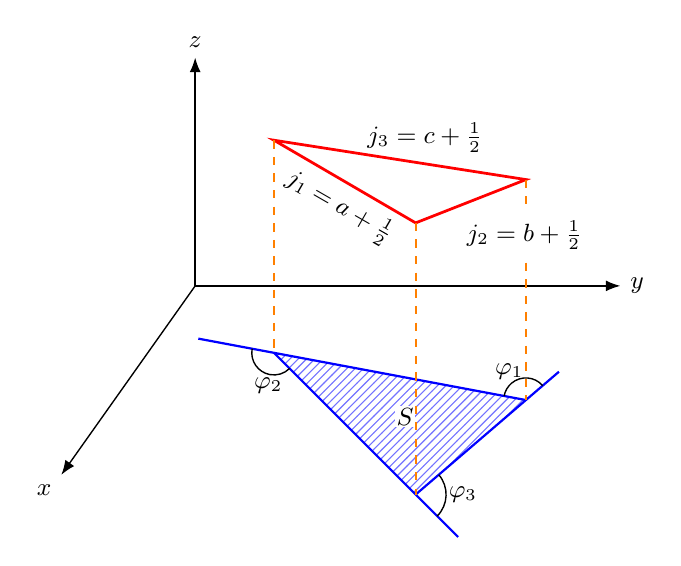
\begin{tikzpicture}[>=Latex,line width=0.5pt,font=\small]
  % --- coordinate axes ---
  \coordinate (O) at (0,0);
  \draw[->] (O) -- (0,2.9)   node[above]{$z$};
  \draw[->] (O) -- (5.4,0)   node[right]{$y$};
  \draw[->] (O) -- (-1.7,-2.4) node[below left]{$x$};
  % --- space triangle (momenta j_i), floating above ---
  \coordinate (A) at (1.0,1.85);   % top-left  vertex
  \coordinate (B) at (4.2,1.35);   % top-right vertex
  \coordinate (C) at (2.8,0.80);   % near/front vertex (lower)
  % --- ground triangle: projection onto (x,y)-plane, area S ---
  \coordinate (PA) at (1.0,-0.85);
  \coordinate (PB) at (4.2,-1.45);
  \coordinate (PC) at (2.8,-2.65);
  \coordinate (PBs) at ($(PC)!1.3!(PB)$);
  \coordinate (PCs) at ($(PA)!1.3!(PC)$);
  \coordinate (PAs) at ($(PB)!1.3!(PA)$);
  \draw[line width=1pt,color=red] (A)--(B)--(C)--cycle;
  \fill[pattern=north east lines,pattern color=blue!55] (PA)--(PB)--(PC)--cycle;
  \draw[thick,color=blue] (PB)--(PAs);
  \draw[thick,color=blue] (PC)--(PBs);
  \draw[thick,color=blue] (PA)--(PCs);
  \node[fill=white,inner sep=0.6pt] at ($(PA)!0.5!(PB)!0.34!(PC)$) {$S$};
  % --- projected exterior angles phi_i ---
  \pic[draw,angle radius=8pt]{angle=PBs--PB--PA};
  \pic[draw,angle radius=8pt]{angle=PAs--PA--PC};
  \pic[draw,angle radius=11pt]{angle=PCs--PC--PB};
  % --- vertical droplines connecting each vertex to its projection ---
  \draw[dashed,thick,color=orange] (A)--(PA);
  \draw[dashed,thick,color=orange] (B)--(PB);
  \draw[dashed,thick,color=orange] (C)--(PC);
  \node at ($(PA)+(-100:0.42)$) {$\varphi_{2}$};
  \node at ($(PB)+(120:0.42)$)  {$\varphi_{1}$};
  \node at ($(PC)+(0:0.60)$) {$\varphi_{3}$};
  \node[above]      at ($(A)!0.6!(B)+(0,0.02)$) {$j_{3}=c+\tfrac12$};
  \node[below,rotate=-30] at ($(A)!0.55!(C)$)              {$j_{1}=a+\tfrac12$};
  \node[below right=1pt,fill=white]  at ($(B)!0.65!(C)$)         {$j_{2}=b+\tfrac12$};
  \end{tikzpicture}
\end{document}